\section{Design principle}

\subsection{What type of problems are GLB applicable to}
GLB is applicable to problems described as following. There is an initial
bag (multiset) of {\em tasks} (may be of size one). A task usually has a
small amount of associated state, but is permitted to access
(immutable) ``reference state''  that can be replicated across all
places. Consequently, tasks are {\em relocatable}: they can be
executed at any place. 

Tasks can be executed. Executing a task may only involve local,
self-contained work (no communication). During execution, a task is
permitted to create zero or more tasks, and produce a result of a given
(pre-specified) type \code{Z}. The user is required to specify a
reduction operator of type \code{Z}. 

The GLB framework is responsible for distributing the generated
collection of tasks across all nodes. Once no more tasks are left to
be executed, the single value of type \code{Z} (obtained by reducing
the results produced by all tasks) is returned.  

Since the execution of each task depends only on the state of the
task (and on immutable external state), the set of results produced on
execution will be the same from one run to another, regardless of
how the tasks are distributed across places. Since the user supplied
reduction operator is assumed to be associative and commutative, the
result of execution of the problem is determinate. Thus GLB is a
determinate application library that requires the user to provide a
few sequential pieces of code and handles concurrency, distribution
and communication automatically. 

The GLB framework is applicable to a wide variety of tasks. For a
simple example, consider the problem of computing the $n$'th Fibonacci
number in the naive recursive way. Here the state of the task can be
summarized by just one number (long), i.e.{} $n$. Execution of the
task yields either a result (for $n < 2$), or two tasks (for $n-1$ and
$n-2$). The results from all tasks need to be reduced through
arithmetic addition. 

All {\em state space search algorithms} from AI fall in the GLB problem domain. Such algorithms are characterized by a space of states, an
initial state, and a generator function which given a state generates
zero or more states. The task is to enumerate all states (perhaps with
a cutoff), apply some function, and combine the results. An example of
such an application is the famous $N$-Queens problem.

\subsection{Execution overview}
Figure ~\ref{fig:design:glb} shows the overall flow of GLB. 
For each GLB program, users need to provide two pieces of sequential code \textit{TaskQueue} and \textit{TaskBag}. In addition, users can also provide an \textit{Initialization} method that tells GLB how to initialize the workload at a root place if the workload cannot be statically scheduled among all places. 

\textit{TaskQueue} embodies the sequential computation for this problem and a result reduction function. \textit{TaskBag} embodies the task container's data structure and its split/merge method.    

Given the \textit{TaskQueue} and \textit{TaskBag} implementation, GLB initializes the workload for each \textit{Worker}. Workers are GLB internal computing/load-balancing engines and they are transparent to GLB users. \textit{Workers} process task items by call the \code{process} method provided by \textit{TaskQueue}. \textit{Workers} balance workload using the lifeline based work-stealing algorithm. GLB splits \textit{TaskBag}s from victim \textit{Worker} and merges them to thief \textit{Worker} by calling the \code{split/merge}  methods provided by \textit{TaskBag}. Once all workers finish working, GLB invokes the \code{reducer} function, provided by \textit{TaskQueue}, to return the final result.

\begin{figure}
\centering
%% 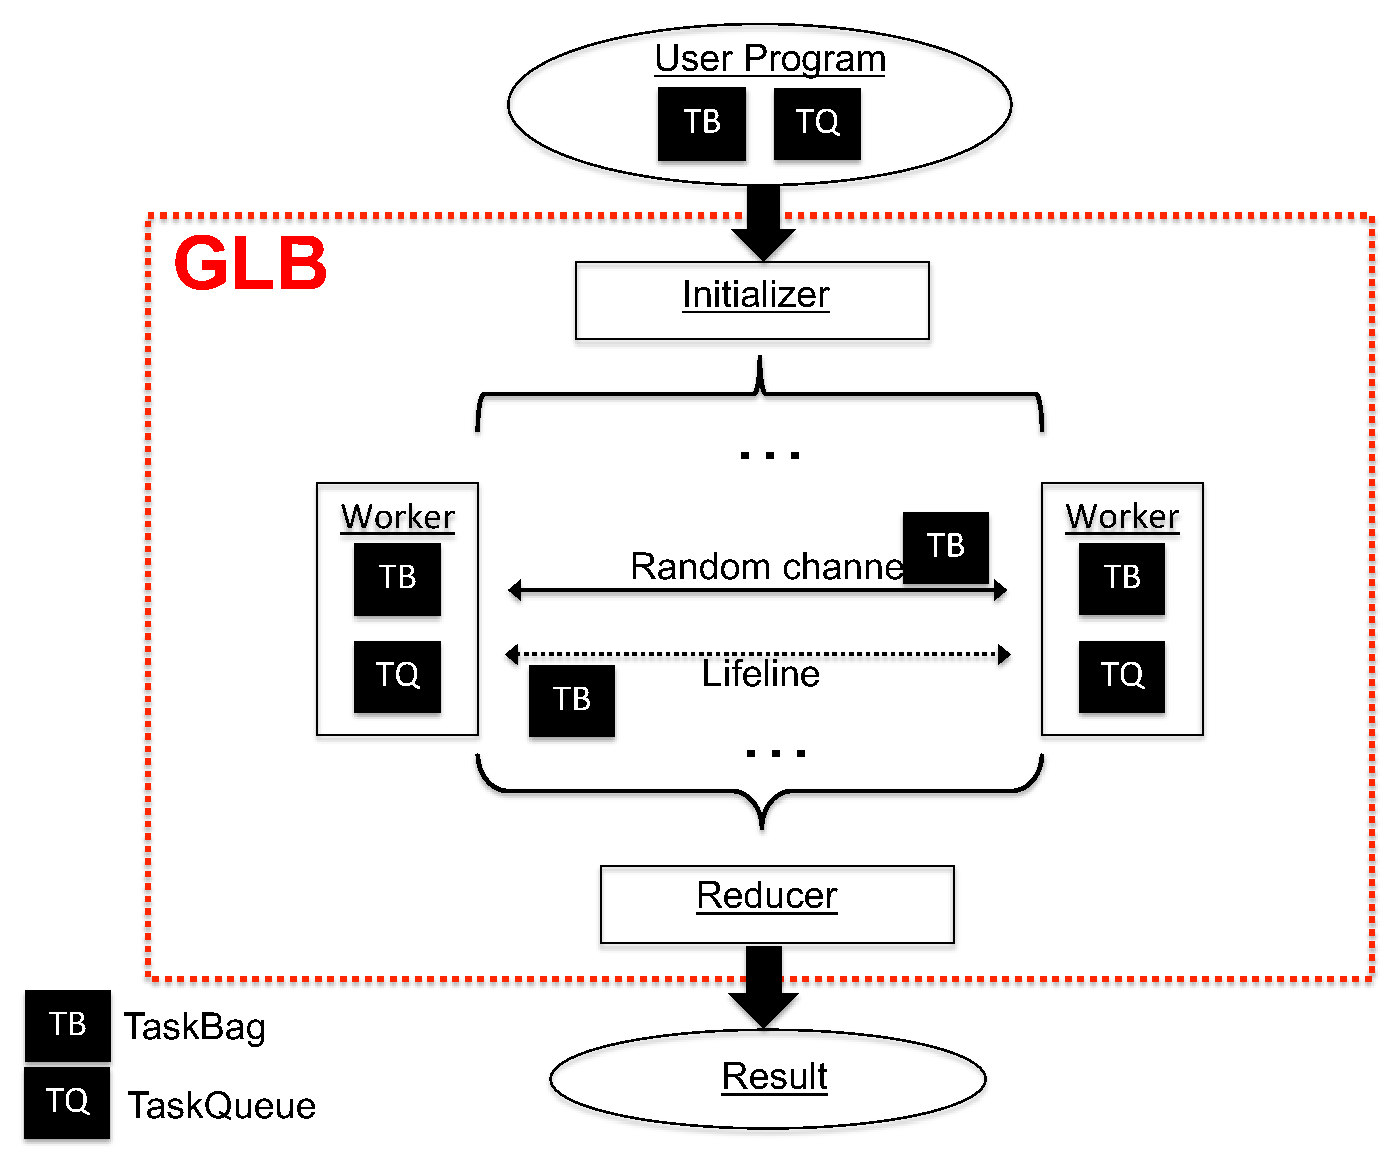
\includegraphics[width=3.25in]{./ppaa2014_figures/glb_overview.eps}
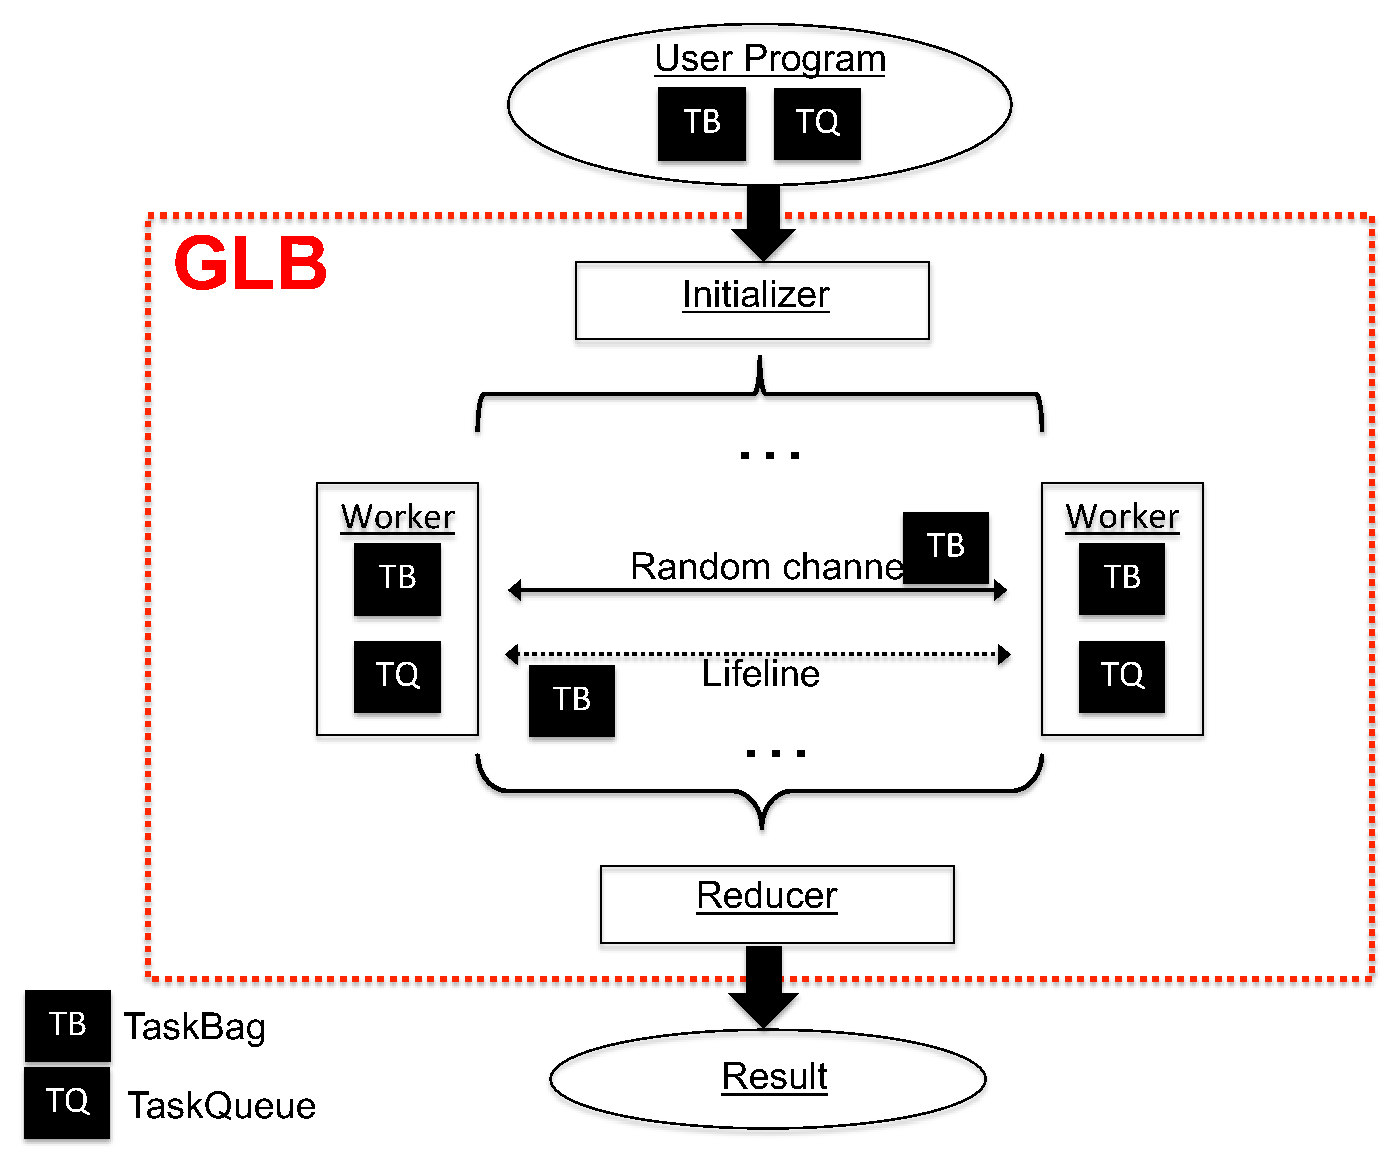
\includegraphics[scale=0.3]{./ppaa2014_figures/glb_overview.eps}
\caption{GLB overview}
\label{fig:design:glb}
\end{figure}


In the following sections, Section~\ref{sec:design:user} discusses what are required from users, Section~\ref{sec:design:internals} discusses the GLB internals, Section~\ref{sec:design:uts} discusses how to apply GLB to the UTS problem, Section~\ref{sec:design:bc} discusses how to apply GLB to the BC problem.


\subsection{What do users need to provide}
\label{sec:design:user}
\textbf{TaskQueue} Users need to provide an implementation of following methods:
\begin{enumerate}
\item \code{process(n:Long):Boolean} This method describes the sequential computation of the problem. It iterates over \textit{n} items in its TaskBag and computes each one of them. It processes $n$ items if available and returns true; otherwise it processes all available ($<n$) items and returns false. When GLB sees a Worker's process(n) returns false, it will schedule this Worker to steal from others.
 \item \code{split():TaskBag} Split its TaskBag and returns the split half. This method returns null if the TaskBag is too small to split.  
\item \code{merge(TaskBag)} Merge the incoming TaskBag to its own TaskBag.
Both split and merge method functions are wrapper functions that will call TaskBag's split/merge functions. 
\item \code{getResult()} Returns local result.
\item \code{reduce()} Result reduction function. Applying this function to each Worker's result yields the final result.
\end{enumerate}
\textbf{TaskBag} Users need to provide a custom class extending \textit{TaskBag} and appropriately implementing \code{split} and \code{merge} methods. They provide the functionalities that \textit{TaskQueue}'s \code{split/merge} methods need. GLB provides a default ArrayList-based TaskBag implementation. In this default implementation, split method is implemented by removing half of the elements from the end of the ArrayList and returning this removed half ArrayList; merge method is implemented by adding all the elements from the incoming ArrayList to the local ArrayList.  


Once the customized TaskQueue and TaskBag are implemented, it is fairly easy for
users to invoke GLB library by calling GLB's \code{run} method. If the workload cannot be statically scheduled across places, users need to provide an \code{initialize} method so that GLB will initialize this root task at place 0.  

\subsection{GLB internals}
\label{sec:design:internals}
GLB implements the lifeline work-stealing algorithm described in \cite{glb}. We summarize the algorithm here:
\begin{enumerate}
\item
Each Worker repeatedly calls \code{process(n)} method until it is running out of work. Between each process(n) call, Worker probes the network and responds to the stealing requests from other Workers. 
\item
When running out of work, a Worker conducts two rounds of work-stealing. It first chooses at most \textit{w} random victims. If none of the random victims has work to share, then Worker goes to the second round of work-stealing by stealing from its life-line buddies/victims. The topology of life-line communication graph is a $z$-dimensional hyper-cube. Such a topology satisfies these properties: it is a fully connected directed graph (so
work can flow from any vertex to any other vertex) and it has a low
diameter (so latency for work distribution is low) and has a low
degree (so the number of buddies potentially sending work to a dead
vertex is low). If a lifeline buddy cannot satisfy the stealing request due to its lack of work, it will still remember the request and try to satisfy the request when it gets work from others.   
\item
When all Workers run out of work, GLB terminates and applies the reduce function to each Worker's result to yield the final result.
\end{enumerate}

Users can tune the GLB performance by changing these parameters:
\textit{w}, \textit{z}, and \textit{n}. It is more likely to steal
work from a random victim with a larger $w$. It is more likely to
steal work from a lifeline buddy when $z$ is larger. However, when $w$
and $z$ get larger, each worker spends more time probing the network and less time in processing tasks. Alternatively, users can make a Worker spend more time on processing tasks by increasing $n$. The larger $n$ is, the more tasks a Worker needs to finish before it can respond to the stealing requests. However, a large $n$ can sometimes hurt the performance if stealing requests need be responded fast. We will see an extreme case in which even $n=1$ is too large a task-granularity in Section~\ref{sec:design:bc}.

To help users understand and tune GLB program performance, GLB also provides logging functionalities to record (1) how much time each Worker spent on processing and distributing work (2) how many (random/lifeline) stealing requests each Worker sent and received. (3) how many (random/lifeline) stealings each Worker perpetrated. (4) How much workload has each Worker received/sent.

To better illustrate how to use GLB, we show a pedagogical use case via the Fibonacci problem in the Appendix.



\subsection{UTS}
\label{sec:design:uts}
\subsubsection{Problem statement}
The Unbalanced Tree Search benchmark measures the rate of traversal of
a tree generated on the fly using a splittable random number
generator. For this submission, we used a \emph{fixed geometric law}
for the random number generator with branching factor $b_0=4$, seed
$r=19$, and tree depth $d$ varying from 13 to 20 depending on core counts and architecture.

\begin{quote}
The nodes in a geometric tree have a branching factor that follows a
geometric distribution with an expected value that is specified by the  
parameter $b_0 > 1$. The parameter $d$ specifies its maximum depth
cut-off, beyond which the tree is not allowed to grow ... The expected
size of these trees is $(b_0)^d$, but since the geometric distribution
has a long tail, some nodes will have significantly more than $b_0$
children, yielding unbalanced trees. 
\end{quote}

The depth cut-off makes it possible to estimate the size of the trees
and shoot for a target execution time. To be fair, the distance from
the root to a particular node is never used in our benchmark
implementation to predict the size of a subtree. In other words, all
nodes are treated equally, irrespective of the current depth.  

%% \subsubsection{Design}

%% The material in this section is excerpted from \cite{glb}, and
%% unchanged from our 2012 HPCC submission.

%% One common way to load balance is to use {\em work-stealing}. For
%% shared memory system this technique has been pioneered in the Cilk
%% system.  Each worker maintains a double ended queue (deque) of tasks. When a
%% worker encounters a new task, it pushes its continuation onto the
%% bottom of the deque, and descends into the task. On completion of the task, it
%% checks to see if its deque has any work, if so it pops a task (from the
%% bottom) and continues with the work. Else (its deque is empty) it
%% looks for work on other workers' deques. It randomly determines a {\em
%%   victim} worker, checks if its queue is non-empty, and if so, pops a
%% task from the top of the deque (the end other than the one being
%% operated on by the owner of the deque).  If the queue is empty, it
%% guesses again and continues until it finds work. Work-stealing systems
%% are optimized for the case in which the number of steals is much
%% smaller than the total amount of work. This is called the ``work
%% first'' principle -- the work of performing a steal is incurred by the
%% thief (which has no work), and not the victim (which is busy
%% performing its work). 

%% Distributed work-stealing must deal with some additional
%% complications. First, the cost of stealing is usually significantly
%% higher than in the shared memory case. For many systems, the target
%% CPU must be involved in processing a steal attempt. Additionally, one
%% must solve the distributed termination detection problem. The system
%% must detect when all workers have finished their work, and there is no
%% more work. At this point all workers should be shut down, and the
%% computation should terminate. 

%% X10 already offers a mechanism for distributed termination detection
%% -- \texttt{finish}. Thus, in principle it should be possible to spawn
%% an activity at each place, and let each look for work. To trigger
%% \texttt{finish} based termination detection however, these workers
%% must eventually terminate. But when? One simple idea is that a worker
%% should terminate after $k$ steal attempts have failed. However this
%% leaves open the possibility that a worker may terminate too early --
%% just because it happened to be unlucky in its first $k$ guesses. If
%% there is work somewhere else in the network then this work
%% can no longer be shared with these terminated workers, thereby
%% affecting parallel efficiency. (In an extreme case this could lead to
%% sequentialize significant portion of the work.) 

%% Therefore there must be a way by which a new activity can be launched 
%% at a place whose worker has already terminated. This leads to the idea
%% of a {\em lifeline graph}. For each place $p$ we pre-determine a set of
%% other places, called {\em buddies}. Once the worker at $p$ has
%% performed $k$ successive (unsuccessful) steals, it examines its
%% buddies in turn. At each buddy it determines whether there is some
%% work, and if so, steals a portion. However, if there is no work, it
%% records at the buddy that $p$ is waiting for work. If $p$ cannot find
%% any work after it has examined all its buddies, it dies -- the place $p$
%% now becomes quiescent.  

%% But if $P$ went to a buddy $B$, and $B$ did not have any work, then
%% it must itself be out looking for work -- hence it is possible that it
%% will soon acquire work. In this case we require that $B$ {\em
%%   distribute} a portion of the work to those workers that attempted to
%% buddy steal from it but failed. Work must be spawned on its own
%% \texttt{async} -- using the \texttt{at (p) async S} idiom. If $P$ had
%%  no activity left, it now will have a fresh activity. Thus, unlike
%%  pure work-stealing based systems, a system with lifeline graphs will
%%  see its nodes moving from a state of processing work (the active state), to a state in
%%  which they are stealing to a state in which they are dead, to a state
%%  (optionally) in which they are woken up again with more work (and are
%%  hence back in the active state).  

%% Note that when there is no work in the system, all places will be dead,
%% there will be no active \texttt{async} in the system and hence the
%% top-level \texttt{finish} can terminate. 

%% The only question left is to determine the assignment of buddies to a
%% place. We are looking for a directed graph that is fully connected (so
%% work can flow from any vertex to any other vertex) and that has a low
%% diameter (so latency for work distribution is low) and has a low
%% degree (so the number of buddies potentially sending work to a dead
%% vertex is low).  $z$-dimensional hyper-cubes  satisfy these properties
%% and have been implemented. 

%% \subsubsection{Implementation}\label{sec:uts-inline}
%% Our implementation follows from \cite{glb} and includes the
%% performance improvements described in our HPCC 2012 submission
%% (using \code{FINISH\_DENSE} to reduce the overhead of termination
%% detection), using \code{@Uncounted} asyncs,  and using a compact
%% representation of the active nodes in a place using an implicit (lower,
%% upper) bounds representation rather than an explicit enumeration.

%% We have made a change in how the native SHA1 code is integrated into
%% X10. Consequently we replaced all of the 169 lines of very complex C++ wrapper code
%% with 3 native annotations (i.e., 3 lines of C code embedded into X10) as for instance in:

%% {\small
%% \begin{verbatim}
%% def this(seed:Int, depth:Int) {
%%   @Native("c++", "rng_init((RNG_state*)this, seed);") {}
%%   this.depth = depth;
%% }
%% \end{verbatim}
%% }

%% We fixed a nasty deadlock condition when using multi-dimensional lifeline graphs.


%% \subsubsection{Verification}
%% The code was validated by checking the results for specific
%% configurations against pre-computed numbers. 


%% % Runs on MPI now ... were there any issues here?
%% \subsubsection{UTS-GLB}\label{sec:utsg}
%% UTS-G is a variant of UTS written using the GLB library. The code for
%% \code{GlobalLoadBalancer} and \code{LocalJobRunner} is no longer
%% needed, since they are part of the library. The code for managing bags
%% of tasks is refactored into a \code{UTSTaskBag} class. Similarly the
%% code for executing a UTS task \code{runATMostNTasks} in
%% \code{UTSTaskFrame} is similarly very straightforward.  The native
%% code (for SHA1 hashes) remains unchanged -- it belongs in the
%% application and not the library.

%% Thanks to the GLB library the number of X10 LOCs drops from 493 for UTS to 225 for UTS-G.

%% %% \subsection{Performance}
%% %% \begin{figure}
%% %% \centering
%% %% \includegraphics[width=3.25in]{figures/p7ih/uts-p7ih.eps}
%% %% \caption{X10 Performance for UTS (on Power~775)}
%% %% \label{fig:perf:uts-p7ih}

%% %% \includegraphics[width=3.25in]{figures/bgq/uts-bgq.eps}
%% %% \caption{X10 Performance for UTS (on Blue~Gene/Q)}
%% %% \label{fig:perf:uts-bgq}

%% %% \includegraphics[width=3.25in]{figures/k/uts-k.eps}
%% %% \caption{X10 Performance for UTS (on K)}
%% %% \label{fig:perf:uts-k}
%% %% \end{figure}

%% %% We report performance for UTS and UTS-G.

%% %% On Power~775, as we demonstrated in our 2012 HPCC Submission, UTS achieves linear speedup up to 50,000 cores. UTS-G is only marginally slower.

%% %% On Blue~Gene/Q and K however, we ran the code ``as is'' without having the time to tune the main parameters of the load balancer to the specifics of the architecture. These parameters include the mapping of the lifeline graph onto the network axes (especially the dimensionality) as well as the frequency of network probes. With proper tuning, we believe we can redress the curves dramatically. In essence, with our implementation and our 2012 runs at scale on Power~775, we established that the benchmark (for this family of trees at least) is compute bound.

%% %% On Blue~Gene/Q, the sequential performance of the UTS-G code is 15\% less than the UTS code: the higher-order implementation confuses the optimizer of the backend compiler (xlC). This is not the case on other platforms. As a result, UTS-G appears to scale better than UTS, but this is misleading.
%% %% At scale, they are more or less on par as UTS only achieves 60\% efficiency for now. Hence the sequential inefficiency of UTS-G can hide behind the latency of the load balancer.

%% %% The measurements on K are very preliminary. The code runs and computes correct results. The performance is under investigation.



%% %We discuss the performance together with UTS-G in Section~\ref{sec:utsg}.
%% %\todo{Performance analysis. Why are numbers bad for the K. Is
%% %  there some basic operation that is slow on the K?}

Clearly, UTS is a case that static load-balancing does not work.  Assume the sequential implementation of UTS is available (i.e., the code to grow the UTS tree and count the nodes), we now discuss how to apply GLB to it.
\subsubsection{UTS TaskBag and TaskQueue }
\textbf{UTS TaskBag} The internal representation of a UTS tree node is a triple(descriptor, low, high). Descriptor represents the hashed value of the node, low represents the smallest index of un-explored children, high represents the largest index of its un-explored children. The representation of a UTS tree is thus an array of UTS tree nodes.
 A UTS TaskBag is essentially a UTS tree. To split a UTS TaskBag, we evenly split each UTS node $n(d,l,h)$ to two nodes $n1(d,l,h1)$ and $n2(d,h2,h)$, where $h1$ and $h2$ are the middle points of $(l,h)$.  If none of the UTS tree node has more than one child node, then we do not split the tree, as it is cheaper to count the node locally than move it to a remote place and count it there. To merge a UTS TaskBag, we simply concatenate the incoming TaskBag's UTS node array to the local one.

\textbf{UTS TaskQueue} \code{process(n)} method counts at most $n$ UTS tree nodes. \code{reduce()} is a straightforward sum-reduction method on each place's UTS tree node count.

Finally, GLB initializes the workload by initializing the root UTS tree node at Place 0.

\subsection{BC}
\label{sec:design:bc}
\subsubsection{Problem statement}
% BC
The Betweenness Centrality benchmark is taken from the SSCA2 (Scalable
Synthetic Compact Application 2) v2.2 benchmark \cite{SSCA2};
specifically, we implement the ``fourth'' kernel in this benchmark,
the computation of {\em betweenness centrality}:

\begin{quotation}
The intent of this kernel is to identify the set of vertices in the
graph with the highest betweenness centrality score. Betweenness
Centrality is a shortest paths enumeration-based centrality
metric, introduced by Freeman (1977). This is done using a betweenness
centrality algorithm that computes this metric for every vertex in the
graph. Let $\sigma_{st}$ denote the number of shortest paths between
vertices $s$ and $t$, and $\sigma_{st}(v)$ the number of those paths
passing through $v$. Betweenness Centrality of a vertex $v$ is defined
as $BC(v) = \Sigma_{s\not=v\not=t \in V} \sigma_{st}(v)/\sigma_{st}$.

The output of this kernel is a betweenness centrality score for each
vertex in the graph and the set of vertices the highest betweenness
centrality score.
\end{quotation}

We implement the Brandes' algorithm described in the benchmark,
augmenting Dijkstra's single-source shortest paths (SSSP) algorithm,
for unweighted graphs. We have implemented the exact variant of the benchmark
(\code{K4approx=SCALE}). 

The solution we implement makes one very strong assumption: that the
graph is ``small'' enough to fit in the memory of a single
place. Since the graph itself is not modified during the execution of
this benchmark, it thus becomes possible to implement this benchmark
by replicating the graph across all places. Now effectively the
computation can be performed in an embarrassingly parallel fashion. The
set of $N$ vertices is statically partitioned among $P$ places; each place is
responsible for performing the computation for the {\em source}
vertices assigned to it (for all $N$ target vertices) and computes its
local \code{betweennessMap}. After this is
done an \code{allReduce} collective performs an \code{AND} summation
    across all local \code{betweennessMaps}. 

Clearly, statically partitioning the work amongst all places in this
way is possible but not ideal. The amount of work associated with one source node
$v$ vs another $w$ could be dramatically different. Consider for
instance a degenerate case: a graph of $N$ vertices, labeled $1\ldots
N$, with an edge $(i,j)$ if $i < j$. Clearly the work associated with
vertex $1$ is much more than the work associated with vertex $N$. 

We next discuss how to dynamically load-balance these
tasks across all places using the GLB framework. 

%% \subsubsection{Structure of the code}
%% The multi-place structure of this code is quite straightforward. We
%% use the standard at-scale X10 idiom for SPMD code:
%% \begin{enumerate}
%% \item Create a distributed data structure, accessed through a
%%   \code{PlaceLocalHandle} which points to an instance of a ``host''
%%   object (an instance of \code{SSCA2}) at each node. (Invocation of
%%   \code{makeFlat}.) 
%% \item Run the actual computation (invocation of \code{broadcastFlat}
%%   with the closure specifying the work to be done at each place.

%%   The work done in each place is the computation of a
%%   \code{bfsShortestPaths} for a slice of vertices from
%%   \code{startVertex} to \code{endVertex}. This loops through the
%%   vertices in the given range, computing the betweennessMap
%%   locally. 

%%   Note this computation is single threaded. It is not difficult to
%%   make this multi-threaded. 

%% \item Once the local computation has been done, and the local
%%   contribution to the betweennessMap computed, a
%%   \code{Team.WORLD.allreduce} ensures that the results are reduced and
%%   made available at place $0$. 
%% \end{enumerate}

%% \subsection{Validation.}
%% The benchmark calls for validating the algorithms by running it on a
%% graph (a torus)  with known analytical results for the betweenness
%% centrality.  Because of lack of time, we have not been able to do
%% this. If our submission is selected for presentation, we plan to
%% validate the algorithm by the time of the presentation.


%% \subsection{Performance measurement.}
%% We discuss the performance together with BC-G in Section~\ref{sec:bcg}.


\subsubsection{BC TaskBag and TaskQueue}
\textbf{TaskBag} Each vertex interval is a task item. We use a tuple(low, high) to represent a vertex interval. Each task bag is an array of such tuples. To split a TaskBag, we divide each tuple evenly. To merge a BC taskbag, we simply concatenate the incoming TaskBag's array to the local one.  

\textbf{TaskQueue} \code{process(n)}  method iterates over the taskbag and calculates the first n vertices. 
\textbf{reduce()} method is a simple betweenness-map (a vector) element-wise add function.

This implementation achieves linear speedup and perfect scalability on
small-scale machines (i.e., 256 cores on Power) for smaller
graph. However, it does not yield equally impressive performance on larger machines for larger graphs. After examining the GLB log, we realized that on large scale machines, Workers are less responsive to the stealing requests thus workload cannot be distributed fast. Therefore, we tried to maximize $w$ and $z$ and minimize $n$. (Please refer to Section~\ref{sec:design:internals} for the rationale of turning these parameters). The performance only improved slightly.
We then realized that it took a Worker too long before it responded to the work stealing requests even when its task granularity is \textbf{one} vertex. So we changed the code that computes each vertex to an interruptable state machine. In this way, a Worker can respond to stealing requests without completing one vertex computation. Alternatively, we can help users to minimize the code change by providing a yielding functionality in the GLB library. Users can insert yield points in the their code to increase its probing frequency and responsiveness to stealing requests. We plan to provide such functionality in GLB in the future work.

